\documentclass[11pt]{report}

\usepackage{epsf,amsmath,amsfonts}
\usepackage{graphicx}
\usepackage{moreverb}
\usepackage{placeins}

\begin{document}

\title{Performance Tuning: \\
Requirements and Design}
\author{Doug Jacobsen, Phil Jones}

\maketitle
\tableofcontents

%-----------------------------------------------------------------------

\chapter{Summary}

This document contains the requiremens and design specifications for use while
optimizing MPAS. The overall outcome of this document will be a version of MPAS
that has a higher level of parallelism available to users, as well as a more
modular design. To begin requirements regarding parallelism are laid out,
followed by requirements for the modularity of the code and potential
enhancements that could be performed at a later time.

%-----------------------------------------------------------------------

\chapter{Requirements}

\section{Performance Portability}
Date last modified: 2011/09/01 \\
Contributors: (Doug Jacobsen, Phil Jones) \\

The MPAS-Ocean code should be performance portable, meaning the code is not optimized for a specific archetecture. All optimized code should remain general, and as readable as possible.  Should any architecture-specific implementations be necessary, there should be generic abstractions that can be confined to a small number of isolated modules that can be selected at compile time.  This may be required, for example, in initial accelerated systems where standards and abstractions have not yet been developed.  Portability in general requires adherence to both language standards and widely-used libraries whenever possible with non-standard approaches again isolated using conditional compilation or preprocessing.

\section{Parallelism}
Date last modified: 2011/09/01 \\
Contributors: (Doug Jacobsen, Phil Jones) \\

Three levels of parallelism will be implemented in MPAS-Ocean, encompassing everything from broad scale parallelism down do accelerated architectures. The three levels can be thought of as follows.

\begin{itemize}
	\item Distributed Memory Parallelism - MPI
	\item Shared Memory Parallelism - OpenMP
	\item Accelerated Architecture Parallelism - TBD (Cuda, OpenCL)
\end{itemize}

\section{Scalability}
Date last modified: 2011/09/01 \\
Contributors: (Doug Jacobsen, Phil Jones) \\

MPAS-Ocean must achieve high scalability appropriate for a given problem size.  Near-linear scalability up to a tens of horizontal grid points per processing element is desired.  For future exascale machines, as many as a billion processing elements may be required, so exposing as much parallelism as possible is desired.  

\section{Modularity}
Date last modified: 2011/09/01 \\
Contributors: (Doug Jacobsen, Phil Jones) \\

The modularity of MPAS-Ocean is to be enhanced to improve readability, enable encapsulation, and simplify the implementation of new parameterizations. Modules will include error feedback to be used for error checking.

\section{Encapsulation}
Date last modified: 2011/09/01 \\
Contributors: (Doug Jacobsen, Phil Jones) \\

Encapsulation within MPAS-Ocean is highly desired.  Encapsulation refers to keeping data and operators local and private within a module whenever possible and only exposing (making public) the interfaces or data needed by calling routines.  This practice helps to prevent namespace conflicts and inadvertant side effects (e.g. a module inadvertantly writing into another array that should not be public). In addition, this practice helps to reduce the overall memory footprint.

%-----------------------------------------------------------------------

\chapter{Design and Implementation}

\section{Performance Portable}
Date last modified: 2011/09/01 \\
Contributors: (Doug Jacobsen, Phil Jones) \\

Performance optimizations will be implemented using standard general techniques. These techniques will include things like loop fusing and removing branching statements within loops. Another general rule of thumb that memory operations (load/stores) are more expensive than flops and that future memory available to each processing element is likely to decrease, implying that temporary arrays should be avoided and overall memory use minimized. 

Loop fusing can be seen in the following context, although there are more examples of this.

\begin{verbatimtab}
do iEdge=1,nEdges
	cell1 = cellsOnEdge(1,iEdge)
	cell2 = cellsOnEdge(2,iEdge)
	do k=1,nVertLevels
		flux = u(k,iEdge) * dvEdge(iEdge) * h_edge(k,iEdge)
		tend_h(k,cell1) = tend_h(k,cell1) - flux 
		tend_h(k,cell2) = tend_h(k,cell2) + flux 
	end do
end do
do iCell=1,nCells
	do k=1,nVertLevels
		tend_h(k,iCell) = tend_h(k,iCell) / areaCell(iCell)
	end do
end do
\end{verbatimtab}

Which can be re-written as

\begin{verbatimtab}
do iEdge=1,nEdges
	cell1 = cellsOnEdge(1,iEdge)
	cell2 = cellsOnEdge(2,iEdge)
	invArea1 = 1.d0 / areaCell(cell1)
	invArea2 = 1.d0 / areaCell(cell2)
	do k=1,nVertLevels
		flux = u(k,iEdge) * dvEdge(iEdge) * h_edge(k,iEdge)
		tend_h(k,cell1) = tend_h(k,cell1) - flux * invArea1
		tend_h(k,cell2) = tend_h(k,cell2) + flux * invArea2
	end do
end do
\end{verbatimtab}

and thus avoids the second loop over nCells*nVertLevels. Also the division is replaced with a less expensive multiply to save on the nVertLevels loop. \\
\\
The removal of branching statements can be seen below:

\begin{verbatimtab}
do iEdge=1,nEdges
  cell1 = cellsOnEdge(1,iEdge)
  cell2 = cellsOnEdge(2,iEdge)

  do k=1,maxLevelEdgeTop(iEdge)

    d2fdx2_cell1 = 0.0
    d2fdx2_cell2 = 0.0

    do iTracer=1,num_tracers

      !-- if not a boundary cell
      if(boundaryCell(k,cell1).eq.0.and.boundaryCell(k,cell2).eq.0) then

        d2fdx2_cell1 = deriv_two(1,1,iEdge) * tracers(iTracer,k,cell1)
        d2fdx2_cell2 = deriv_two(1,2,iEdge) * tracers(iTracer,k,cell2)

        !-- all edges of cell 1
        do i=1, grid % nEdgesOnCell % array (cell1)
          d2fdx2_cell1 = d2fdx2_cell1 &
		      + deriv_two(i+1,1,iEdge) &
		      * tracers(iTracer,k,grid % CellsOnCell % array (i,cell1))
        end do

        !-- all edges of cell 2
        do i=1, grid % nEdgesOnCell % array (cell2)
          d2fdx2_cell2 = d2fdx2_cell2 & 
		      + deriv_two(i+1,2,iEdge) &
		      * tracers(iTracer,k,grid % CellsOnCell % array (i,cell2))
        end do
      endif

      flux = dvEdge(iEdge) *  u(k,iEdge) * h_edge(k,iEdge) * (          &
         0.5*(tracers(iTracer,k,cell1) + tracers(iTracer,k,cell2))      &
         -(dcEdge(iEdge) **2) * (d2fdx2_cell1 + d2fdx2_cell2) / 12. )

      !-- update tendency
      tend_tr(iTracer,k,cell1) = tend_tr(iTracer,k,cell1) - flux/areaCell(cell1)
      tend_tr(iTracer,k,cell2) = tend_tr(iTracer,k,cell2) + flux/areaCell(cell2)
    enddo
  end do
end do
\end{verbatimtab}

which can be replaced with

\begin{verbatimtab}
do iEdge=1,nEdges
  cell1 = cellsOnEdge(1,iEdge)
  cell2 = cellsOnEdge(2,iEdge)


  do k=1,maxLevelEdgeTop(iEdge)

    d2fdx2_cell1 = 0.0
    d2fdx2_cell2 = 0.0
    boundaryMask1 = (.not. boundaryCell(k,cell1) ) * 1.d0
    boundaryMask2 = (.not. boundaryCell(k,cell2) ) * 1.d0

    do iTracer=1,num_tracers
      d2fdx2_cell1 = deriv_two(1,1,iEdge) &
		  * tracers(iTracer,k,cell1)      &
		  * boundaryMask1
      d2fdx2_cell2 = deriv_two(1,2,iEdge) &
		  * tracers(iTracer,k,cell2)      &
		  * boundaryMask2

      !-- all edges of cell 1
      do i=1, grid % nEdgesOnCell % array (cell1)
        d2fdx2_cell1 = d2fdx2_cell1     &
               + deriv_two(i+1,1,iEdge) &
             * tracers(iTracer,k,grid % CellsOnCell % array (i,cell1)) &
             * boundaryMask1
      end do

      !-- all edges of cell 2
      do i=1, grid % nEdgesOnCell % array (cell2)
        d2fdx2_cell2 = d2fdx2_cell2     &
               + deriv_two(i+1,2,iEdge) &
             * tracers(iTracer,k,grid % CellsOnCell % array (i,cell2)) &
             * boundaryMask2
      end do

      flux = dvEdge(iEdge) *  u(k,iEdge) * h_edge(k,iEdge) * (          &
         0.5*(tracers(iTracer,k,cell1) + tracers(iTracer,k,cell2))      &
         -(dcEdge(iEdge) **2) * (d2fdx2_cell1 + d2fdx2_cell2) / 12. )

      !-- update tendency
      tend_tr(iTracer,k,cell1) = tend_tr(iTracer,k,cell1) - flux/areaCell(cell1)
      tend_tr(iTracer,k,cell2) = tend_tr(iTracer,k,cell2) + flux/areaCell(cell2)
    enddo
  end do
end do
\end{verbatimtab}

Which replaces the branch with 6 multiplies and two logicial not statements, and allows the loop to be vectorized easier. Other performance enhancements are to be implemented as seen fit.

\section{Parallelism}
Date last modified: 2011/09/01 \\
Contributors: (Doug Jacobsen, Phil Jones) \\

In order to implement the three levels of parallelism, code requires a variety of modifications. The distrubuted memory parallelism is already implemented using MPI commands, but some optimization for these can be explored. 

OpenMP (or other threading paradigm) is necessary on computers with multi-core CPU's, especially as core counts per node increase.  MPI implementations across cores can often result in bus contention if the vendor has not optimized for local shared memory. However, an appropriate OpenMP implementation will require some experimentation.  If enough subdomains are assigned to an MPI task, OpenMP parallelism may be desireable at a high level in the code, threading over subdomains similar to distributed memory parallism.  Alternatively, directives can be added around loops and where it appears to be useful. Care must be taken to evaluate the approaches and identify ways of maintaining data locality with the threads (often vendors provide some capability at run time, though may require care if ``first touch'' is a mechanism for pinning memory).  

The third level of parallelism will take the most work. To begin, a suitable method of parallization for accelerated architectures needs to be identified. In the event CUDA or OpenCL are chosen to perform a set of tasks on GPUs some major modifications will need to be done to algorithms suitable for programing in this fashion, at least if portable code is still a major goal. 

In order to maintain portable code and use CUDA or OpenCL it is likely that some algorithms, or modules, will need to be ported to having a Fortran interface on top of C code, to allow the use of multiple compilers. CUDA is currently only supported with the use of the PGI Fortran compiler and OpenCL is not supported in Fortran at all. As we explore these specific implementations, suitable abstractions may become apparent and these abstractions can call specific CUDA or OpenCL code underneath.  This is a significant research area at present. 
.


\FloatBarrier
\section{Modularity}
Date last modified: 2011/09/01 \\
Contributors: (Doug Jacobsen, Phil Jones) \\

In order to aid the parallel development of MPAS-Ocean by multiple developers, and increase overall performance of MPAS-Ocean, the modularity of MPAS-Ocean will be increased. Identified components within currently existing portions of code can be extracted and put into their own modules, as seen fit.

As an example, within module\_time\_integration.F the horizontal mixing of tracers and momentum has a $\nabla^2$ and $\nabla^4$ option hard coded. This would be removed, and put in it's own module named something like module\_OcnHmixMom.F. This module would include possible parameterizations, and handle the selection of each. In the described case two sub-modules would be created each named something like module\_OcnHmixMomDel2.F and module\_OcnHmixMomDel4.F, representing each of the two options. Each of these would contain the portion of code relevant to computing the tendencies for the momentum equation related to the parameterization.

This modular programming fashion allows several things.  First, it allows parameterizations to be explored and implemented in an easier fashion than is currently available in MPAS-Ocean.  Second, the pointers inherent in the current MPAS data structures and registry present a barrier to compiler optimization.  By modularizing tendency calculations, it is possible to pass pointers into arrays so that compilers at the module level can optimize the underlying array code while retaining the flexibility of the pointers and structures at the top levels and for configuration. 
Third, it should reduce the overall memory footprint of the MPAS-Ocean at any point in time, as only the arrays required by the current modules will be allocated. And finally, it increases the ability for encapsulation within MPAS-Ocean.


Modularity can be seen in figure \ref{fig:modules}.  This figure is only a conceptual figure at present and will be replaced by a more detailed module layout soon.

\begin{figure}
	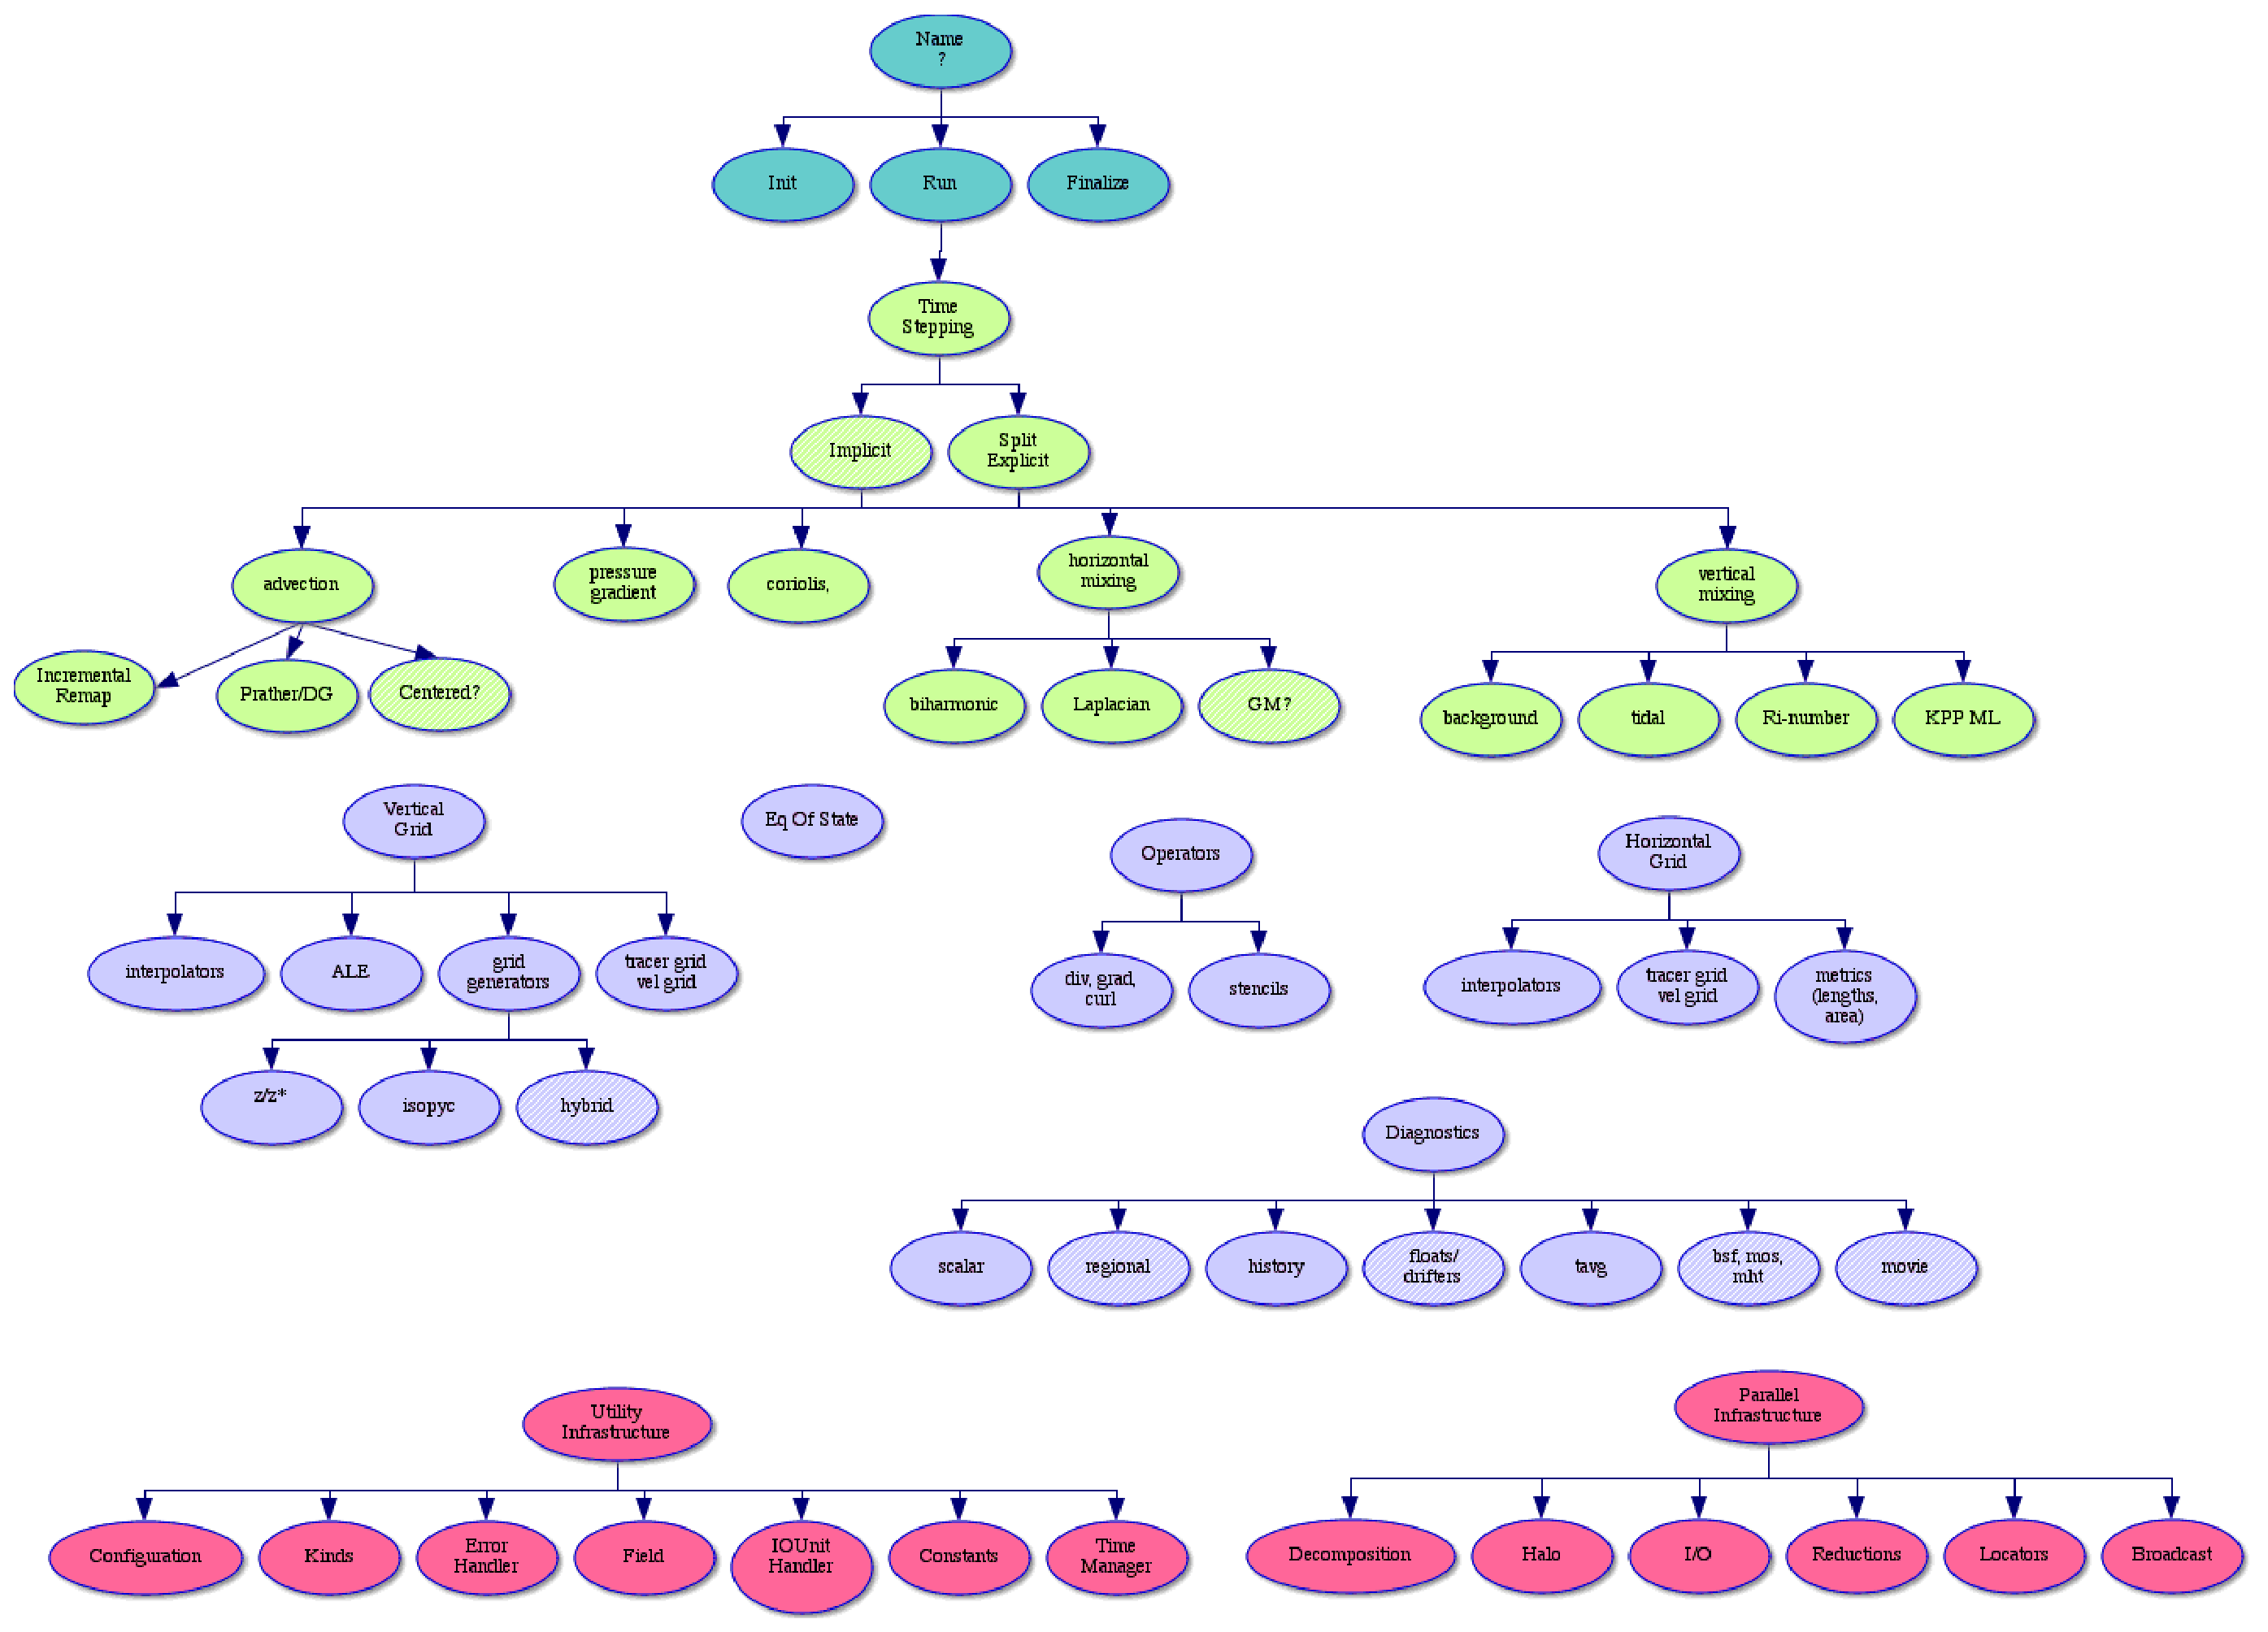
\includegraphics[scale=0.35]{NewArchitecture.eps}
	\label{fig:modules}
	\caption{Example of proposed modularity of MPAS-Ocean.}
\end{figure}

\FloatBarrier
\section{Encapsulation}
Date last modified: 2011/09/01 \\
Contributors: (Doug Jacobsen, Phil Jones) \\

Encapsulation is currently implemented by making all module variables and interfaces private by default (with a private statement in the module header).  Only data or interfaces that need to be public are given the public attribute.  In addition, most modules will contain their own initialization routine to initialize module variables and options.  In the future, current registry variables will need to reflect the module granularity of input namelist options.

%-----------------------------------------------------------------------

\chapter{Testing}
\section{Testing and Validation}
Date last modified: 2011/09/01 \\
Contributors: (Doug Jacobsen, Phil Jones) \\

Testing of each performance enhancement will be explored by using a basic set of timers and test cases. Unit tests will be developed that can then be set as part of a suite of tests useful for further development. Some larger tests will also be used to verify the models accuracy, and that no detrimental changes were made in each step.

A useful effort would be to develop a ``test'' suite that can be run on a branch or trunk to validate the output of the current model. Ideally this would be a script that could be submitted to an HPC queue, and would run several test cases and examine the results to determine if the model is correct or not. Of course the test cases and criteria for a ``correct'' model need to be determined.

%-----------------------------------------------------------------------

\end{document}
